\documentclass[10pt]{beamer}
\usepackage[utf8]{inputenc}
\usepackage{subcaption}
\usepackage{soul}
\usepackage{tikz}
\usetikzlibrary{shapes}
\usepackage{pgfplots}
\usetheme{Madrid}
%\usecolortheme{seahorse}
\colorlet{beamer@blendedblue}{red!6!green!33!blue}
\usefonttheme[onlylarge]{structurebold}
\setbeamerfont*{frametitle}{size=\normalsize,series=\bfseries}
\setbeamertemplate{navigation symbols}{}


\title{Introduction à l'apprentissage statistique}
\author{Par Esp\'eran Padonou} 
\institute[EEIA]{
      \includegraphics[width=0.36\textwidth, height=0.14\textwidth]{
      {figures/LOGO EEIA.png}}
}

\titlegraphic{
\includegraphics[width=0.15\textwidth, height=0.15\textwidth]{{figures/logoFV.jpg}}
\hspace{0.1\textwidth}
\includegraphics[width=0.15\textwidth, height=0.15\textwidth]{{figures/Fondation_de_France.png}}
\hspace{0.1\textwidth}
   \includegraphics[width=0.15\textwidth, height=0.15\textwidth]{{figures/logoBE.png}}
   \hspace{0.1\textwidth}
   \includegraphics[width=0.075\textwidth, height=0.15\textwidth]{{figures/UNDP-LOGO.pdf}}
   
}

\date[Godomey 2024]{ \\  Godomey, le 29 juillet 2024 }


\newcommand{\Comment}[1]{
  \smallskip\par\noindent{\color{blue}$\rightarrow$ #1}
}
\newcommand{\myblue}[1]{\textcolor{blue}{#1}}
\newcommand{\myor}[1]{\textcolor{orange}{#1}}
\newcommand{\myviolet}[1]{\textcolor{violet}{#1}}
\newcommand{\Cellp}[2]{
  \setlength{\fboxsep}{2pt}\setlength{\fboxrule}{0pt}%
  \framebox{\parbox{#1}{
      \color{black}{#2}}}  
}


\AtBeginSection{
\begin{frame}
    \begin{centering}
    \begin{beamercolorbox}[sep=12pt,center]{part title}
	{\huge
    \usebeamerfont{section title}\insertsection\par}
    \end{beamercolorbox}
    \end{centering}
\end{frame}
}
 

\begin{document}
\maketitle

%%%%%%%%%%%%%%%%%%%%%%%%%%%%%%%%%%%%%%%%%%%%%%%%%%%%%%
\begin{frame}
\frametitle {Le machine learning}

\begin{block}{Définition ?}
\small {\begin{itemize}
\item Apprentissage automatique
\item Apprentissage artificiel
\item Apprentissage statistique
\item Statistical learning   
\item Simulation de l'intelligence humaine
\item Ou d'une certaine intelligence animale ?
\end{itemize}}
\end{block}
 

\begin{minipage}{\textwidth}
\vspace{0.1\textwidth}
\centering
 \textbf{Ingrédients:  Mathématiques, statistiques, probabilités, algorithmique.}
\end{minipage}
\end{frame}


%%%%%%%%%%%%%%%%%%%%%%%%%%%%%%%%%%%%%%%%%%%%%%%%%%%%%%
\begin{frame}{Problème 1 : détecter un événement exceptionnel}
\vskip 0.05\linewidth
\begin{minipage}{0.6\textwidth}
\begin{tabular}{|*{15}{c|}}
    \hline
     11& 12& 11& 16& 12& 11& 10& 8&  19& 15& 11& 15& 14& 10& 11 \\
     \hline 
     12& 14& 10& 15& 12& 13& 12& 13& 13& 11& 14&  9& 16& 13& 10\\
    \hline
\end{tabular}
\end{minipage}
\begin{center}

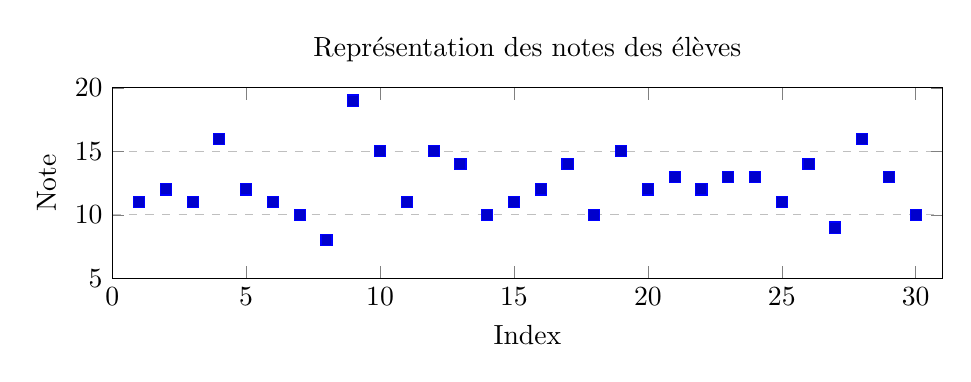
\begin{tikzpicture}
    \begin{axis}[
    title={Représentation des notes des élèves},
    width = \textwidth,
    height = 4cm,
    xmin=0, xmax=31,
    ymin=5, ymax=20,
    ymajorgrids=true,
    grid style=dashed,
    xlabel = Index,
    ylabel = {Note}
    ]
    \addplot+[only marks,
    mark=square*
    ] coordinates {
        (1,11) (2,12) (3,11) (4,16) (5,12) (6,11) (7,10)        (8,8) (9,19) (10,15) (11,11) (12,15) (13,14) (14,10) (15,11)        (16,12) (17,14) (18,10) (19,15) (20,12) (21,13) (22,12)        (23,13) (24,13) (25,11) (26,14)  (27,9) (28,16) (29,13) (30,10)
    };
    \end{axis}
\end{tikzpicture}

\begin{block}{Y a-t-il une note exceptionnelle ? }
\begin{itemize}
\item Comment la définissez-vous ? \pause 
\item Comment un ordinateur peut-il la retrouver ? Règle, formule ? 
\end{itemize}
\end{block}
\end{center}
\end{frame}
%%%%%%%%%%%%%%%%%%%%%%%%%%%%%%%%%%%%%%%%%%%%%%%%%%%%%%

\begin{frame}{Problème 2 : optimisation} 
\begin{minipage}{0.45\textwidth}
\begin{block}{Où positionner une antenne}
\small {\begin{itemize}
\item Avec quel objectif ? 
\item Quelles variables ? 
\item Quelle stratégie ?
\item Quelles contraintes ? 
\end{itemize}}
\end{block}
\end{minipage}
\begin{minipage}{0.53\textwidth}
\begin{center}
\includegraphics[height=1.2\textwidth]{figures/antenne0.jpg}
\end{center}
\end{minipage}
\end{frame}

%%%%%%%%%%%%%%%%%%%%%%%%%%%%%%%%%%%%%%%%%%%%%%%%%%%%%%

\begin{frame}{Problème 3 : classification} 
 \begin{center}
\includegraphics[height=0.4\textwidth]{figures/knn_question.png}
\end{center} 
 
\begin{block}{Trouver le couleur du nouveau point}
\small {\begin{itemize}
\item En sachant sa position
\item En sachant les couleurs des anciens points 
\end{itemize}}
\end{block} 

\end{frame}

%%%%%%%%%%%%%%%%%%%%%%%%%%%%%%%%%%%%%%%%%%%%%%%%%%%%%%

\begin{frame}{Problème 3 : classification} 
 
\begin{center}
\includegraphics[height=0.4\textwidth]{figures/knn_solution1.png}
\end{center} 
 
\begin{block}{Algorithme des k plus proches voisins}
\small {\begin{itemize}
\item Calculer des distances 
\item Les classer par ordre croissant
\item Retenir les k plus petites valeurs et compter 
\end{itemize}}
\end{block} 
\end{frame}

%%%%%%%%%%%%%%%%%%%%%%%%%%%%%%%%%%%%%%%%%%%%%%%%%%%%%%

 
 \begin{frame}{Problème 3 : choisir k} 
 
\begin{center}
\includegraphics[height=0.4\textwidth]{figures/knn_comparaison.png}
\end{center} 
 
\begin{block}{Vers la sélection de modèles}
\small {\begin{itemize}
\item Comment évaluer le cas k = 3 ? 
\item Des idées... 
\end{itemize}}
\end{block} 
\end{frame}

%%%%%%%%%%%%%%%%%%%%%%%%%%%%%%%%%%%%%%%%%%%%%%%%%%%%%%

 \begin{frame}{Problème 3 : exercice} 
 
\begin{center}
\includegraphics[height=0.4\textwidth]{figures/Prix_terrains.png}
\end{center} 
 
\begin{block}{Prix de vente de terrains dans une zone convoitée de Cotonou}
\small {\begin{itemize}
\item Modifiez l'algorithme (sortie quantitative et même aire). 
\item Variations horizontales VS variations verticales : commentez. Idées ?
\item Idées si les surfaces sont différentes ? Pour différentes années de vente.
\end{itemize}}
\end{block} 
\end{frame}

%%%%%%%%%%%%%%%%%%%%%%%%%%%%%%%%%%%%%%%%%%%%%%%%%%%%%%

\begin{frame}{Problème 4 : l'analyse multivariée} 
 
\begin{block}{Contrôle de gestion}
\small {\begin{itemize}
\item Quantité de canne à sucre achetée (tonnes) : $MP \in [0,  30]$ 
\item Quantité de sucre fabriqué (caisses) : $PF \in [0,  30]$
\item Redressement fiscal bien que $MP$ et $PF$ soient dans leur intervalle historique
\end{itemize}}
\end{block} \pause
\begin{center}
\includegraphics[height=0.4\textwidth]{figures/acp0.png}
\end{center} 
 
\end{frame}
%%%%%%%%%%%%%%%%%%%%%%%%%%%%%%%%%%%%%%%%%%%%%%%%%%%%%%

\begin{frame}{Problème 4 : l'analyse multivariée} 
 
\begin{block}{Contrôle de gestion}
\small {\begin{itemize}
\item Grand axe : ordre de grandeur de $MP$ et $PF$
\item Petit axe : lien entre $MP$ et $PF$
\item La relation entre les variables devient un indicateur à surveiller
\item Vers l'Analyse en Composantes Principales  
\end{itemize}}
\end{block}  

\begin{center}
\includegraphics[height=0.4\textwidth]{figures/acp2.png}
\end{center} 
\end{frame}

%%%%%%%%%%%%%%%%%%%%%%%%%%%%%%%%%%%%%%%%%%%%%%%%%%%%%%
\begin{frame}{Problème 5 : Régression} 
\hspace{-0.12\textwidth}
\begin{minipage}{0.45\textwidth}
 \begin{center}
\includegraphics[height=\textwidth]{figures/data_coiffeur.PNG}
\end{center} 
\end{minipage}
\begin{minipage}{0.53\textwidth}
\begin{center}
\includegraphics[height=1\textwidth]{figures/reg0.png}
\end{center}
\end{minipage}

\begin{itemize}
    \item Que dire des prix pratiqués par ce coiffeur ? 
    \item Quel est le prix probable pour 10 personnes ?
\end{itemize}

\end{frame}
%%%%%%%%%%%%%%%%%%%%%%%%%%%%%%%%%%%%%%%%%%%%%%%%%%%%%%


\begin{frame}{Problème 5 : Régression} 
\hspace{-0.12\textwidth}
\begin{minipage}{0.45\textwidth}
 \begin{center}
\includegraphics[height=\textwidth]{figures/data_coiffeur.PNG}
\end{center} 
\end{minipage}
\begin{minipage}{0.53\textwidth}
\begin{center}
\includegraphics[height=1\textwidth]{figures/reg1.png}
\end{center}
\end{minipage}

 
\begin{itemize}
    \item Définir les moindres carrés
    \item Commentez le choix $a = -100$
\end{itemize}

\end{frame}
%%%%%%%%%%%%%%%%%%%%%%%%%%%%%%%%%%%%%%%%%%%%%%%%%%%%%%

\begin{frame}{Problème 5 : Régression} 
\hspace{-0.12\textwidth}
\begin{minipage}{0.45\textwidth}
 \begin{center}
\includegraphics[height=\textwidth]{figures/data_coiffeur.PNG}
\end{center} 
\end{minipage}
\begin{minipage}{0.53\textwidth}
\begin{center}
\includegraphics[height=1\textwidth]{figures/reg2.PNG}
\end{center}
\end{minipage}
\end{frame}

%%%%%%%%%%%%%%%%%%%%%%%%%%%%%%%%%%%%%%%%%%%%%%%%%%%%%%

\begin{frame}{Problème 5 : Régression} 
\hspace{-0.12\textwidth}
\begin{minipage}{0.45\textwidth}
 \begin{center}
\includegraphics[height=\textwidth]{figures/data_coiffeur.PNG}
\end{center} 
\end{minipage}
\begin{minipage}{0.53\textwidth}
\begin{center}
\includegraphics[height=1\textwidth]{figures/reg3.PNG}
\end{center}
\end{minipage}
\end{frame}

%%%%%%%%%%%%%%%%%%%%%%%%%%%%%%%%%%%%%%%%%%%%%%%%%%%%%%

\begin{frame}{Problème 6 : Paradoxe de Simpson} 
 
 \begin{center}
\includegraphics[height=0.34\textwidth]{figures/SIMPSON_tableau.png}
\end{center} 

\begin{block}{Deux commentaires qui s'opposent}
\small {\begin{itemize}
\item Le directeur : Notre taux de réussite a augmenté de plus de 13\% !
\item Toto : Les redoublants ont moins réussi cette année. \\
            \hspace{0.06\textwidth} Le non-redoublants également ont moins réussi qu'en 2021!
\item Vers les modèles par arbre : un modèle pour les redoublants et un modèle pour les autres. 
\end{itemize}}
\end{block} 

\end{frame}
%%%%%%%%%%%%%%%%%%%%%%%%%%%%%%%%%%%%%%%%%%%%%%%%%%%%%%
\begin{frame}{Problème 6 : Paradoxe de Simpson} 
 
 \begin{center}
\includegraphics[height=0.34\textwidth]{figures/SIMPSON_tableau.png}
\end{center} 

\begin{block}{Deux commentaires qui s'opposent}
\small {\begin{itemize}
\item Le directeur : Notre taux de réussite a augmenté de plus de 13\% !
\item Toto : Les redoublants ont moins réussi cette année. \\
            \hspace{0.06\textwidth} Le non-redoublants également ont moins réussi qu'en 2021!
\item Vers les modèles par arbre : un modèle pour les redoublants et un modèle pour les autres. 
\end{itemize}}
\end{block} 

\end{frame}
%%%%%%%%%%%%%%%%%%%%%%%%%%%%%%%%%%%%%%%%%%%%%%%%%%%%%%
\begin{frame}{Problème 7 : un exemple classique} 

\begin{itemize} 
    \item $x_1$ et $x_2$ sont binaires et $y = x_1 .\mathrm{ XOR }. x_2$
    \item Représentation de $y$ en code couleur dans le plan $(x_1, x_2)$  
\end{itemize}

 \begin{center}
\includegraphics[width=0.4\textwidth]{figures/xor.JPG}%
\hspace{0.15\textwidth}
\includegraphics[width=0.4\textwidth]{figures/représentation.JPG}
\end{center} 

\begin{itemize}
    \item Comment prédire la couleur de l'un des points s'il était inconnu ?%  
          \begin{itemize}
           \item Par les $k$ plus proches voisins ?  
           \item Par régression linéaire ?  
        \end{itemize} 
\end{itemize}
\end{frame}
%%%%%%%%%%%%%%%%%%%%%%%%%%%%%%%%%%%%%%%%%%%%%%%%%%%%%%
\begin{frame}{Problème 7 : un exemple classique} 
 \begin{center}
\includegraphics[width=\textwidth]{figures/regression_xor.JPG} 
\end{center} 

\end{frame}

%%%%%%%%%%%%%%%%%%%%%%%%%%%%%%%%%%%%%%%%%%%%%%%%%%%%%%
 
\begin{frame}{Problème 7 : un exemple classique} 

 \begin{center}
\includegraphics[width=0.6\textwidth]{figures/modèle_final.JPG} 
\end{center} 

\begin{itemize}
           \item Première ligne pour vérifier qu'au moins une valeur vaut 1
           \item Seconde ligne pour vérifier que $x_1$ et $x_2$ ne valent pas 1 à la fois
        \end{itemize} 
 
\end{frame}
%%%%%%%%%%%%%%%%%%%%%%%%%%%%%%%%%%%%%%%%%%%%%%%%%%%%%%
\begin{frame}{Problème 7 : Vers les réseaux de neurones} 

 \begin{center}
\includegraphics[width=0.25\textwidth]{figures/reg_RN.JPG}%
\hspace{0.15\textwidth}
\includegraphics[width=0.4\textwidth]{figures/Perceptron.JPG}
\end{center} 

\begin{itemize}
           \item Introduire dans le modèle de régression des variables intermédiaires, combinant les entrées et influençant la sortie, invisibles à l'entrée et à la sortie du modèle
           \item Un pas vers l'apprentissage profond et les réseaux de neurones  
        \end{itemize} 
 
\end{frame}

%%%%%%%%%%%%%%%%%%%%%%%%%%%%%%%%%%%%%%%%%%%%%%%%%%%%%%
 


\begin{frame}{Problème 8 : Planification d'expériences} 
\begin{minipage}{0.72\textwidth}
\begin{figure} [H] 
\centering
\includegraphics[width=\textwidth, height=0.35\textwidth]{figures/IOT}
\caption*{Connected objects}
\end{figure}
\end{minipage}
\hspace{0.01\linewidth}
\begin{minipage}{0.25\textwidth}
\begin{figure} [H] 
 \centering
\includegraphics[width=\textwidth, height=0.5\textwidth]{figures/ICST.jpg}
\caption*{Integrated circuits}
\end{figure}
\end{minipage}

\begin{minipage}{0.72\textwidth}
\begin{block}{Contexte industriel}
\small {\begin{itemize}
\item Travail en partenariat avec STMicroelectronics. \\ 
      $\Rightarrow$ Production de circuits integrés. \\
      $\Rightarrow$ Supports d'usinage en forme de disques.
\item Haute qualité et contrôles coûteux. \\
      $\Rightarrow$ IA pour le Contrôle de Avancé de Procédés
\end{itemize}}
\end{block}
\end{minipage}
\begin{minipage}{0.25\textwidth}
\vspace{0.1\textwidth}
\begin{figure} [H] 
 \centering
\includegraphics[width=0.7\textwidth, height=0.7\textwidth]{figures/wafer}
\caption*{Un wafer}
\end{figure}
\end{minipage}
\end{frame}
 
\begin{frame} 
\begin{block}{Plans d'expériences adaptés au procédé laser}
\begin{figure}[H] 
\begin{subfigure}[l]{0.2\textwidth}
\centering
\includegraphics[width=\textwidth, height=\textwidth]{figures/doe2.png}
\label{fige}
\end{subfigure}%
\hspace{0.05\textwidth}
\begin{subfigure}[l]{0.2\textwidth}
\centering 
\includegraphics[width=\textwidth, height=\textwidth]{figures/doe3.png}
\label{fige}
\end{subfigure}%
\hspace{0.05\textwidth}
\begin{subfigure}[l]{0.2\textwidth}
\centering 
\includegraphics[width=\textwidth, height=\textwidth]{figures/doe5.png}
\label{fige}
\end{subfigure}%
\hspace{0.05\textwidth}
\begin{subfigure}[l]{0.2\textwidth}
\centering 
\includegraphics[width=\textwidth, height=\textwidth]{figures/doe5bis.png}
\label{fige}
\end{subfigure}%
 
\end{figure}
\end{block} \pause

 
 \begin{block}{Plans d'expériences adaptés au dépôt en phase plasma}
\begin{figure}[H] 
\begin{subfigure}[l]{0.2\textwidth}
\centering
\includegraphics[width=\textwidth, height=\textwidth]{figures/doea.png}
\label{fige}
\end{subfigure}%
\hspace{0.05\textwidth}
\begin{subfigure}[l]{0.2\textwidth}
\centering 
\includegraphics[width=\textwidth, height=\textwidth]{figures/doeb.png}
\label{fige}
\end{subfigure}%
\hspace{0.05\textwidth}
\begin{subfigure}[l]{0.2\textwidth}
\centering 
\includegraphics[width=\textwidth, height=\textwidth]{figures/doec.png}
\label{fige}
\end{subfigure}
\end{figure}
\end{block}

La qualité des données plutôt que la quantité.
\end{frame}


\begin{frame} {Problème 9 : interprétation et connaissance métier}
\vspace{0.01\textwidth}
\begin{figure}[H] 
\begin{subfigure}[l]{0.3\textwidth}
\centering
\includegraphics[width=0.9\textwidth, height=0.56\textwidth]{figures/laserprocess.jpg}
\label{fige}
\end{subfigure}%
\hspace{0.13\textwidth}
\begin{subfigure}[l]{0.3\textwidth}
\centering
%\vspace{0.07\textwidth}
\includegraphics[width=1\textwidth, height=0.6\textwidth]{figures/plasmaCVD.JPG}
\label{fige}
\end{subfigure}%

\begin{subfigure}[l]{0.05\textwidth}
\centering
\includegraphics[width=\textwidth, height=\textwidth]{figures/fleche_bas.png}
\label{fige}
\end{subfigure}%
\hspace{0.37\textwidth}
\begin{subfigure}[l]{0.05\textwidth}
\centering
\includegraphics[width=\textwidth, height=\textwidth]{figures/fleche_bas.png}
\label{fige}
\end{subfigure}%

\begin{subfigure}[l]{0.3\textwidth}
\centering
\includegraphics[width=0.65\textwidth, height=0.6\textwidth]{figures/profil_laser.png}
\label{fige}
\end{subfigure}%
\hspace{0.13\textwidth}
\begin{subfigure}[l]{0.3\textwidth}
\centering
\includegraphics[width=0.66\textwidth, height=0.6\textwidth]{figures/profil_cvd.png}
\label{fige}
\end{subfigure}%
\end{figure}

\begin{block}{Grande variété de formes, due aux procédés d'usinage}
\setbeamertemplate{itemize items}[triangle]
\begin{itemize}
\item Les données, mais aussi les processus sous-jacents. 
\end{itemize} 
\end{block}
\end{frame}
\begin{frame} {Problème 10 : les outils graphiques}
 
\begin{block}{Il ne s'agit pas d'un problème, mais d'une clé!}
\end{block}
\end{frame}
\end{document}

